  \documentclass{article}
   \textwidth = 19cm 
   \oddsidemargin = -1.7cm
   \evensidemargin = -1.4cm

   \usepackage{tikz}
   \usetikzlibrary{calc}
	
   \usepackage{biblatex}
   	
   \begin{document}

   \begin{minipage}{0.23 \textwidth}

   \begin{center}
   \textbf{Le cube}\vskip.3truecm 

   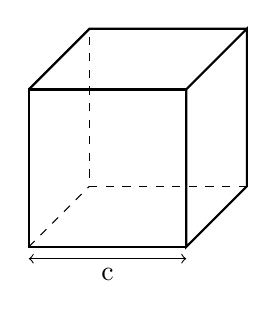
\begin{tikzpicture}[scale=0.5]
   \draw[thick,black] (4,0,0) -- (0,0,0) -- (0,4,0) -- (4,4,0);
   \draw[thick,black]  (4,0,0) -- (4,0,-4) -- (4,4,-4) -- (4,4,0) -- cycle;
   \draw[thick,black](0,4,0) -- (0,4,-4) -- (4,4,-4);
   \draw[style=dashed, color=black] (4,0,-4) -- (0,0,-4)-- (0,4,-4);
   \draw[style=dashed, color=black] (0,0,0) -- (0,0,-4); 
   \draw[<->](0,-0.3,0)--(4,-0.3,0);
   \draw node[below] at (2,-0.3,0) {c}; 
   \end{tikzpicture}

   \vskip.3truecm$Volume =\dotfill $ 
   \end{center}

   \end{minipage}
   \hfill
   \begin{minipage}{0.23\textwidth}

   \begin{center}
   \textbf{Le pav\'e droit} \\
   (parall\'el\'epip\`ede rectangle)\vskip.3truecm

   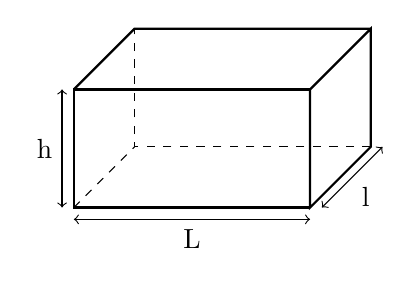
\begin{tikzpicture}[scale=0.5]
   \draw[thick,black] (6,0,0) -- (0,0,0) -- (0,3,0) -- (6,3,0);
   \draw[thick,black]  (6,0,0) -- (6,0,-4) -- (6,3,-4) -- (6,3,0) -- cycle;
   \draw[thick,black](0,3,0) -- (0,3,-4) -- (6,3,-4);
   \draw[style=dashed, color=black] (6,0,-4) -- (0,0,-4)-- (0,3,-4);
   \draw[style=dashed, color=black] (0,0,0) -- (0,0,-4); 
   \draw[<->](-0.3,0,0)--(-0.3,3,0);
   \draw node[left] at (-0.3,1.5,0) {h}; 
   \draw[<->](0,-0.3,0)--(6,-0.3,0);
   \draw node[below] at (3,-0.3,0) {L}; 
   \draw[<->](6.3,0,0)--(6.3,0,-4);
   \draw node[below right] at (6.3,0,-2) {l}; 
   \end{tikzpicture}        

   \vskip.3truecm$Volume =\dotfill $ 
   \end{center}

   \end{minipage}
   \hfill
   \begin{minipage}{0.23 \textwidth}

   \begin{center}
   \textbf{Le prisme droit}\vskip.3truecm

   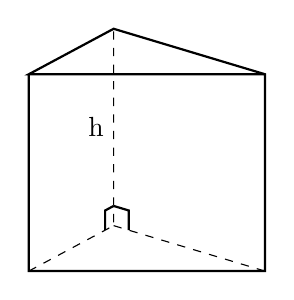
\begin{tikzpicture}[scale=0.5]
   \draw[thick,black] (0,5,0)-- (0,0,0) -- (6,0,0)--(6,5,0)--(1,5,-3)--(0,5,0)--(6,5,0);
   \draw[style=dashed, color=black] (0,0,0) -- (1,0,-3)-- (1,5,-3);
   \draw[style=dashed, color=black]  (1,0,-3)-- (6,0,0);
   \draw[thick,black] (1.5,0,-2.7)  --(1.5,0.5,-2.7)--(1,0.5,-3) ;
   \draw[thick,black] (0.9,0,-2.7)  --(0.9,0.5,-2.7)--(1,0.5,-3) ;
   \draw node[left] at (1,2.5,-3) {h};    
   \end{tikzpicture}


   \vskip.3truecm$Volume =\dotfill $ 
   \end{center}

   \end{minipage}
   \hfill
   \begin{minipage}{0.23 \textwidth}

   \begin{center}
   \textbf{Le cylindre}\vskip.3truecm

   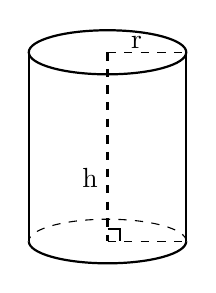
\begin{tikzpicture}[scale=0.8]
   \draw[thick,black](3,0,-2) ellipse (1.25 and 0.35);
   \draw[thick,black]  (1.75,-3,-2) arc (180:360:1.25 and 0.35);
   \draw [dashed]  (4.25,-3,-2) arc (0:180:1.25 and 0.35);
   \draw[style=dashed, color=black](3,-3,-2) -- (4.25,-3,-2);
   \draw[style=dashed, color=black](3,0,-2) -- (4.25,0,-2);          
   \draw node[above left] at (3.7,-0.1,-2) {r}; 
   \draw node[left] at (3,-2,-2) {h}; 
   \draw[thick,black]  (1.75,0,-2) --(1.75,-3,-2);
   \draw[thick,black]  (4.25,0,-2) --(4.25,-3,-2);
   \draw[thick,black] (3,-2.8,-2 ) --(3.2,-2.8,-2 ) --(3.2,-3,-2 );   
   \draw[thick,black, dashed] (3,0,-2)--(3,-3,-2 );
   \end{tikzpicture}


   \vskip.3truecm$Volume =\dotfill $ 
   \end{center}

   \end{minipage}
   \vskip1truecm

   \begin{minipage}{0.3 \textwidth}

   \begin{center}
   \textbf{La pyramide} \vskip.3truecm

   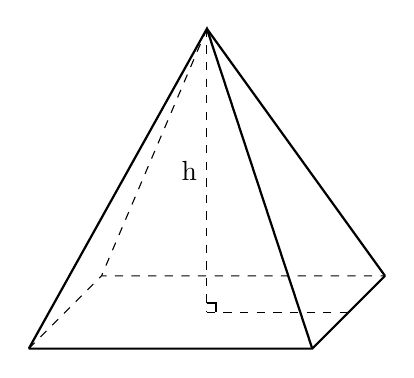
\begin{tikzpicture}[scale=0.6]
   \draw[thick,black] (0,3,0)--(6,3,0)--(6,3,-4);
   \draw[style=dashed, color=black](0,3,0) -- (0,3,-4) -- (6,3,-4);
   \draw[thick,black] (0,3,0) -- (3,9,-2) -- (6,3,0);
   \draw[thick,black]  (3,9,-2) -- (6,3,-4);
   \draw[style=dashed, color=black](3,9,-2) -- (0,3,-4);
   \draw[style=dashed, color=black](3,9,-2) -- (3,3,-2);
   \draw[style=dashed, color=black](3,3,-2) -- (6,3,-2);
   \draw[thick,black] (3,3.2,-2 ) --(3.2,3.2,-2 ) --(3.2,3,-2 );
   \draw node[left] at (3,6,-2) {h};
   \end{tikzpicture}

   \vskip.3truecm$Volume =\dotfill $ 
   \end{center}

   \end{minipage}
   \hfill
   \begin{minipage}{0.3 \textwidth}

   \begin{center}
   \textbf{Le c\^one}  \vskip.3truecm

   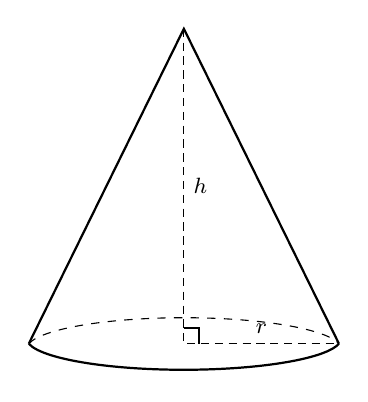
\begin{tikzpicture}
   \draw[dashed] (0,0) arc (170:10:2cm and 0.4cm)coordinate[pos=0] (a);
   \draw[thick,black] (0,0) arc (-170:-10:2cm and 0.4cm)coordinate (b);
   \draw[densely dashed] ([yshift=4cm]$(a)!0.5!(b)$) --node[right,font=\footnotesize] {$h$}coordinate[pos=0.95] (aa)($(a)!0.5!(b)$)-- node[above,font=\footnotesize] {$r$}coordinate[pos=0.1] (bb) (b);
   \draw[thick,black] (aa) -| (bb);
   \draw[thick,black] (a) -- ([yshift=4cm]$(a)!0.5!(b)$) -- (b);
   \end{tikzpicture}


   \vskip.3truecm$Volume =\dotfill $ 
   \end{center}

   \end{minipage}
   \hfill
   \begin{minipage}{0.3 \textwidth}

   \begin{center}
   \textbf{La sph\`ere - La boule}\vskip.3truecm

   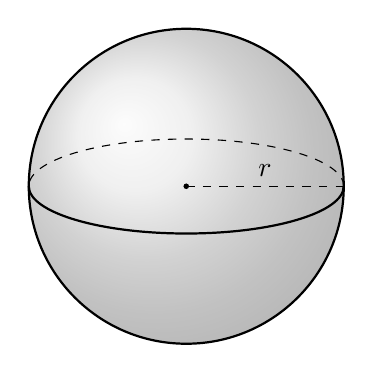
\begin{tikzpicture}
     \shade[ball color = gray!40, opacity = 0.4] (0,0) circle (2cm);
   \draw[thick,black](0,0) circle (2cm);
   \draw[thick,black](-2,0) arc (180:360:2 and 0.6);
   \draw[dashed] (2,0) arc (0:180:2 and 0.6);
   \fill[fill=black] (0,0) circle (1pt);
   \draw[dashed] (0,0 ) -- node[above]{$r$} (2,0);
   \end{tikzpicture}


   \vskip.3truecm$Volume =\dotfill $ 
   \end{center}

   \end{minipage}
   
   \printbibliography
   \end{document}